\section{Prior Work}

Work on Reagent principally concerns bringing together two discrete lines
of work. The first is prior work on building intelligent system that are
capable of combining multimodal input to generate an intent for the user,
which was covered in Section~\ref{sec:cais_prior_work}. On second
line of interest, we look at the rich research on automatic extraction of
information from webpages and the lessons learned there, especially in how
they might work with ontology building. Cimiano et
al.~\cite{cimiano_towards_2004} and Storey et 
al.~\cite{storey_ontology_2005} propose frameworks on parsing
important information from web pages, which would be then encoded into RDF
structures. Gangemi~\cite{gangemi_comparison_2013} provides a recent
overview of available technologies in this space.
However, these approaches generally focus on the use of just natural
language understanding over the entire page for key terms and relations,
and not necessarily leveraging the increasingly rich ways the data may
be shown in a page that require true DOM traversal and analysis. However,
in analysis and automatic parsing of the DOM structure, we are informed
by prior work on taking into account elements that are ``noise'' (e.g.
ads and popups) which might look well-structured, but that the user most
likely does not care about. Gupta et al.~\cite{gupta_dom-based_2003}
utilizes the full DOM-tree to determine relevance of elements.
Joshi and Liu~\cite{joshi_web_2009} utilize both DOM traversal and NLP
to determine salient details. Sun et al.~\cite{sun_dom_2011} utilize a
algorithm that considers content density within nodes. Our current work
focuses on automatic analysis of elements that rarely, if ever, appear
within this ``noisy'' data, but is important to consider as we expand
Reagent to further domains. Finally, in the realm of understanding purely
tabular data, Hackinger~\cite{hackinger_datagorri:_2018} proposes a
system similar in some regards to \textit{Reagent}, but that it requires
for any new site the human to first identify the table on the page and
to present a ``template'' on how it should be parsed, acting far less
autonomously than \textit{Reagent}. These works inform our approach
on building \textit{Reagent}, but it is important to note that our
end-goal, principally in automatic on-the-fly webpage parsing and
ontology building for use in multimodal applications, is different.

\begin{comment}
% this is a slimmed diagram of the one shown in chap 2, so ignored
\begin{figure}
    \centering
    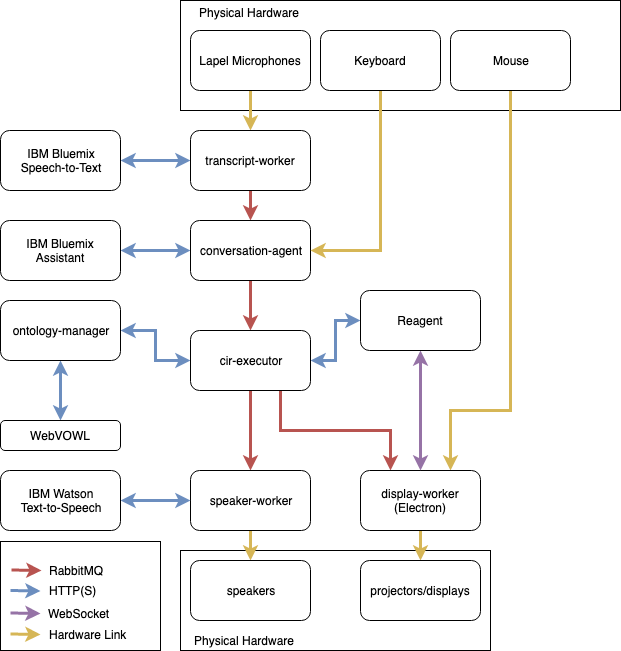
\includegraphics[width=0.45\textwidth]{chapters/03_reagent/figures/cir_diagram}
    \caption{Diagram of the Cognitive and Immersive System for Reagent}
    \label{fig:cais}
\end{figure}
\end{comment}